\chapter{Wstęp}
\label{cha:pierwszyDokument}


Pierwsze obrazy wideo powstały już na początku XX wieku i opierały się na mechanicznie obracających się dyskach. Technologia ta istniała głównie w sferze badań akademickich i nie zdominowała rynku. Dopiero z wprowadzeniem cathode-ray tube (CRT) wraz z telewizją analogową, wideo zaczęło być wykorzystywane komercyjnie. Z czasem rozwój technologii pozwolił na wprowadzenie telewizji cyfrowej, która zapewniała wyższą jakość obrazu oraz lepsze wykorzystanie zasobów. Wideo razem z~audio okazały się również znakomitym środkiem wymiany informacji. Stały się coraz częściej wykorzystywane do komunikacji w czasie rzeczywistym zastępując tradycyjne połączenie telefoniczne w biznesie oraz dla zwykłych użytkowników. Rozwój na rynku telefonów również wspomógł powszechność wideo. W momencie kiedy praktycznie każdy aparat zaczął posiadać kamerę, wideo zaczęło konkurować ze zdjęciami jako metoda na utrwalenie chwili. Codziennie tak rejestrowane obrazy są przekazywane do rodziny, znajomych oddalonych o tysiące kilometrów. Kolejnym przykładem kiedy wideo zastępuje tradycyjne formy przekazu są blogi internetowe. Do tej pory prowadzone na zasadzie artykułów/postów, teraz zaczęły wykorzystywać wideo jako metodę dystrybucji informacji.

Dzięki coraz większym przepustowościom i szerokiemu dostępowi do Internetu w najnowszych czasach wykreował się jeszcze inny trend sprawiający, że obrazy wideo są bardziej popularne. Mowa tu o platformach streamingowych takich jak - YouTube, Netflix czy HBOgo. Pozwalają one użytkownikom na oglądanie od krótkich filmików, przez seriale, po pełnometrażowe filmy nawet w rozdzielczościach 4k. Przewidywane jest, że do 2022, aż 82 procent całego ruchu IP, to będzie wideo \cite{prediction}. \par


%Wszystkie wymienione wyżej aspekty sprawiły, że wideo stało się codziennością w życiu większości ludzi.\par \todo[inline]{To bym usunął, nic nie wnosi i jeszcze dziwnie wygląda jednolinijkowy akapit.}

Na obecnym etapie rozwoju technologii, oczekiwania odbiorcy co do jakości otrzymywanego wideo znacznie wzrosły. Na drugiej szali pozostają ograniczenia dotyczące medium i optymalnego wykorzystania zasobów po stronie klienta i dostawcy. Odnosząc się do powyższego istotną kwestią staje się monitorowanie jakości transmitowanego wideo i dostosowywanie go do potrzeb użytkownika. Jednak problem w ocenie jakości wideo jest o tyle trudny, że dotychczas najbardziej wiarygodnym wskaźnikiem jest tu opinia ludzka,  trudna do powiązania z mierzalnymi technicznymi, parametrami wideo.\par

Przykładem koncepcji poprawy trafności dla automatycznej oceny jakości wideo jest wykorzystanie jednej z gałęzi statystyki -- Uczenia maszynowego. Pomaga ona odnajdywać zależności, nawet te na pozór nie intuicyjne, dla zbioru cech wideo. Tą metodę zastosowano do tej pory podczas tworzenia między innymi metryki VMAF oraz metryk zaproponowanych przez Judith Redi \cite{metryka1} i Patrick'a Le Callet \cite{metryka2}.


W niniejszej Pracy zostanie przedstawiony algorytm pozwalający na bardziej zautomatyzowaną ocenę jakości wideo w oparciu o metryki \emph{full-reference} (FR) i \emph{no-reference} (NR) z użyciem wybranych metod z zakresu uczenia maszynowego oraz zaprezentowana zostanie wykorzystana metodologia badań.


\chapter{Wprowadzenie teoretyczne}
\label{cha:pierwszyDokument}

W niniejszym rozdziale przedstawiono najważniejsze teoretyczne zagadnienia dla przeprowadzonych badań. Opisane one zostały w sposób pozwalający czytelnikowi na odpowiednie zrozumienie dalszej części pracy, pomijając nieistotne szczegóły. Pierwsza część rozdziału dotyczy tematu wideo. Przedstawiono jego definicję, oraz wybrane cechy statystyczne biorące udział w trakcie badań. W kolejnej części zaprezentowano zagadnienia z obszaru uczenia maszynowego. Wyjaśniona została jej ogólna koncepcja, a następnie opisano użyte algorytmy.


\section{Wideo}

Wideo jest formą zapisu sygnału wizji (analogowego bądź cyfrowego). W swojej surowej postaci jest to sekwencja pojedynczych ramek. Ramki natomiast składają się z pikseli, a one są definiowane poprzez: luminancję ({\em ang. luminace}) i chrominancje ({\em ang. chrominance}). Luminancja odpowiada za jasność obrazu, a chrominancja za kolorystykę. 

Surowe wideo zajmuje bardzo dużo przestrzeni dyskowej. Przykładowo obraz o rozdzielczości 1920x1080 z 24 ramkami na sekundę o długości 30 sekund zajmuje ponad \todo{sprawdzić ile dokładnie ((1920x1080x3x24x30/1024)/1024)/1024 ~ 4GB }30 GB w pamięci komputera. Tak duże rozmiary znacząco ograniczają możliwości przechowywania i transmisji dla zwykłych użytkowników. Dlatego praktycznie każdy plik wideo wykorzystuje kodeki, czyli pewne ustandaryzowane zasady kompresji/dekompresji. Do tej grupy należą między innymi: H.261, MPEG-1, H.262/MPEG-2, H.263, H.265 i powszechnie używany w Internecie do transmitowania multimediów --  H.264 \cite{video_codecs}. 

Można wyróżnić dwa rodzaje kompresji: stratna i bezstratna. W przetwarzaniu obrazów stosowana jest ta pierwsza. Kompresja stratna może znacząco obniżyć rozmiar pliku. W przypadku wideo wskaźnik kompresji może wynosić nawet 200:1 \cite{compression_rate}\todo[inline]{Skąd ta liczba?- done}. Technika ta korzysta wtedy z ograniczeń ludzkiego oka i usuwa informacje o obrazie, które mają większą szanse na bycie niewychwyconym.\todo[inline]{To po co algorytmy testowania jakości skoro nikt tego nie wychwytuje?- done}. Poniżej zaprezentowano schemat przetwarzania obrazu stałego kodekiem JPEG.

\tikzstyle{block} = [rectangle, draw, fill=white, text width=6em, text centered, minimum height=5em]

\begin{center}
\begin{figure}
\begin{tikzpicture}[node distance = 4cm, auto] 

\node [block] (sam) {Oryginalny obraz};

\node [block, right of=sam] (var) {Podział na bloki pikseli};

\node [block, right of=var] (pro) {Transformata na dziedzine częstotliwości};

\node [block, below of=pro] (clus) {Kwantyzacja} ;

\node [block, left of=clus] (val) {Kompresja};

\node [block, minimum width=3cm, left of=val] (res) {Skompresowany strumień bitów};

\draw [->] (sam) -- (var);

\draw [->] (var) -- (pro);

\draw [->] (pro) -- (clus);

\draw [->] (clus) -- (val);

\draw [->] (val) -- (res);

\end{tikzpicture}
\centering
\caption{Schemat kodowania dla JPEG.}
\end{figure}
\end{center}


\todo[inline]{Do takiego schematu polecam tikz-a - będzie lepiej wyglądać i łatwiej będzie go edytować. Tu są przykład: - DONE}
Większość kodeków bazuje swoje działanie na transformacji DCT (\emph{ang. Discreet Cosinus Transform}). Polega ona na przeniesieniu, wcześniej wydzielonych z oryginalnego obrazu bloków pikseli, z dziedziny przestrzeni (sygnał obrazu przedstawia się za pomocą macierzy, gdzie jej elementy reprezentują piksele) \todo[inline]{Co to jest dziedzina przestrzeni?- done} do dziedziny częstotliwości. Na tak przygotowanych blokach dokonywana jest kwantyzacja. Proces ten polega na zapisaniu  wartości pikseli na ograniczonej liczbie bitów, co już zmniejsza rozmiar danych. Kolejnym krokiem jest zastosowanie algorytmów kompresji jak na przykład: \emph{run-length coding} i \emph{variable-length coding}. Pierwszy z nich grupuje ciągi zer i zapisuje ich liczbę zamiast całej takiej serii. Drugi zmienia postać słów kodowych na bardziej wydajna formę, poprze zapisanie tych często występujących krótszą sekwencją bitów \cite{kodowanie} (na przykład dzięki kodowaniu Huffman'a). \todo[inline]{Ten proces kompresja stratna obrazu i kompresja bezstratna bitów jakie na koniec otrzymamy, ten opis jest bardzo niedokładny - done ?}

Często pierwszym krokiem przed dokonaniem kompresji jest zmiana kodowania kolorów z systemu RGB na YUV. Na czym polega to kodowanie szerzej omówione jest w podrozdziale dotyczącym cech video.

Kodeki wideo dodatkowo dokonują kompresji na podstawie różnic w ramkach. Dzięki tej technice po kompresji zatrzymane są  pełne dane tylko o części z nich. Do odkodowania pozostałych ramek wystarczą tylko policzone wcześniej różnice \cite{kodowanie}. To rozwiązanie czerpie korzyści przede wszystkim z elementów obrazu, które nie zmieniają się zbyt dynamicznie. \todo[inline]{Nie jest to takie proste, kodujemy różnicę, więc same wektory ruchu nie wystarczą- done }

Ze względu na sposób kodowania można wyróżnić trzy typy ramek.
\begin{itemize}[label=$\bullet$]
	\item I (\emph{ang. intra frame}) -- kodowana jak obrazy stałe.
	\item P -- kodowana na podstawie poprzednich wyświetlonych ramek.
	\item B -- kodowana na podstawie wcześniejszych i późniejszych ramek.
\end{itemize}

\begin{figure}[h]
	\centerline{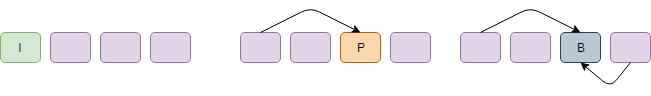
\includegraphics[ height=3cm, width=13cm]{ramki}}
	\caption{Trzy typy kodowania ramek.}
	\label{fig:ramki}
	\label{fig:xccs}
\end{figure}
 

Sam proces kompresji jak i błędy transmisji czy nagrywania mogą powodować powstanie zaburzeń w odtwarzanym obrazie. Przykłady tych niepożądanych efektów opisane zostały w rozdziale 2.2.1. W celu mierzenia poziomu uszkodzeń oraz monitorowania stanu wideo badacze zdefiniowali wiele metryk.\par 

\todo[inline]{Ostatni akapit jest bardzo niezgrabny stylistycznie/gramatycznie. Teraz dowiadujemy się więcej o kompresji, ale nadal nie wiemy tego co najważniejsze, jak wyglądają typowe zniekształcenia, co mają wykrywać nasze metryki?- ? ale czy o tym nie będę pisała więcej poniżej?}

\section{Metryki}
%https://books.google.se/books?id=JbtPCwAAQBAJ&pg=PA32&dq=video++quality+metrics+full+reference&hl=en&sa=X&ved=0ahUKEwi4wtGc2YfiAhWx-ioKHZJtAtcQ6AEIKjAA#v=onepage&q=video%20%20quality%20metrics%20full%20reference&f=false

Referencyjną oceną jakości wideo jest tak zwana ocena subiektywna. Polega ona na określeniu jakości odbioru przez człowieka na podstawie jego odczuć. Niestety, aby takie badanie było miarodajne należy je przeprowadzić w odpowiednich warunkach, przygotować zestaw testów, zrekrutować uczestników oraz cały czas nadzorować jego przebieg. Wszystko to generuje duże koszty i zabiera czas, ale przede wszystkim nie pozwala na ocenę jakości w czasie rzeczywistym na przykład podczas przesyłania wideo w sieci. Problem ten rozwiązują metryki jakości wideo. które w przeciwieństwie do oceny subiektywnej, bazują na obiektywnych pomiarach właściwości obrazu \cite{vqm}.\par

Metryki jakości wideo mogą zostać sklasyfikowane na podstawie tego czy do ich wyznaczenia wymagana jest obecność oryginalnego pliku wideo. Metryki, które wymagają takiego pliku określane są mianem {\em  full-reference} (FR). Porównują one właściwości zniekształconego i bazowego wideo, aby na podstawie tak otrzymanych informacji dokonać estymaty jakości. Innym rodzajem metryk są metryki {\em no-reference} (NR). Dokonują one oceny jakości na podstawie tylko zniekształconego wideo i nie wymagają do tego żadnych dodatkowych informacji \cite{vqm}.\par



Podczas badań nad jakością  wideo używane są pewne sformułowania ułatwiające definiowanie późniejszych pojęć. Przedstawiają się one następująco:
\begin{itemize}[label=$\bullet$]
	\item SVQ (\emph{ang. Subjective video quality}) -- jakość wideo odbierana przez człowieka
	\item SRC (\emph{ang. Source}) -- oryginalna sekwencja wideo
	\item PVS (\emph{ang. Processed Video Sequences}) -- pliki wideo powstałe w skutek zniekształcenia SRC
\end{itemize}
\todo[inline]{Typowym zabiegiem jest przeniesienie sekcji słownika jako osobny rozdział na początku pracy, w tym miejscu jest to dziwne, bo nawet nie korzysta Pani z tych pojęć w ``okolicy''.}

W poniższych podrozdziałach w skrócie zostały opisane metryki typu NR i FR.

\subsection{Metryki no-reference}
%\let\labelitemi\labelitemii
\begin{itemize}[label=$\bullet$]
\item Blokowość ({\em ang. Blockiness}) -- powstaje podczas kodowania. Dotyczy związanych z tym procesem bloków pikseli i kompresji jaka jest na nich dokonywana. Objawia się poprzez zauważalną między tymi blokami granicę\cite{blockiness}. \todo[inline]{Czegoś w tym zdaniu brakuje- done} Skala przyjęta w pracy: 0-3570. Im większa wartość, tym mniej widoczne zakłócenie\cite{agh_vqm}. \todo[inline]{Nic z tego opisu nie rozumiem. Skala jest to 3570, ale już od 0.9 nic nie widać, to po co wartości > 1?- rzeczywiście dziwne, ale to jest informacja z źródła od naszej katedry - http://vq.kt.agh.edu.pl/metrics.html, ale najwyraźniej coś tu jest nie tak:) -  usunełam zbędny fragment- Done }
% Dla obrazu bez zakłóceń około 0.9-1.01 
\begin{figure}[h]
\centerline{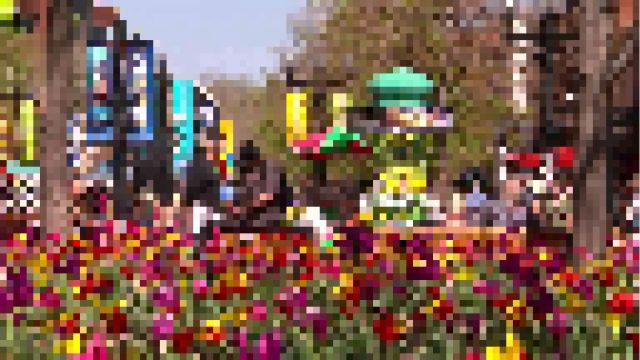
\includegraphics[ height=4cm, width=7cm]{blockiness}}
\caption{Przykładowy obraz z zakłóceniami spowodowanymi blokowością \cite{agh_vqm}.}
\label{fig:xccs}
\end{figure}

\item Aktywność przestrzenna ({\em ang. Spatial Activity}) -- opisuje położenie obiektu na ramce oraz jego relacje z innymi obiektami. Pozwala rozróżnić czy aktywność na danym wideo jest czynnością statyczną (przykładowo: osoba wykonująca czynność pozostaje w jednym miejscu) czy mobilną (przykładowo: osoba wykonująca czynność porusza się wzdłuż pola widzenia) \cite{spactial_act}. Skala przyjęta w pracy: 0-270. Im większa wartość, tym większa aktywność przestrzenna \cite{agh_vqm}. \todo[inline]{po co tu jakieś osoby, jak się będzie ruszać kamera a nie osoby to nie będzie wartości? - DONE?}
\begin{center}
\centerline{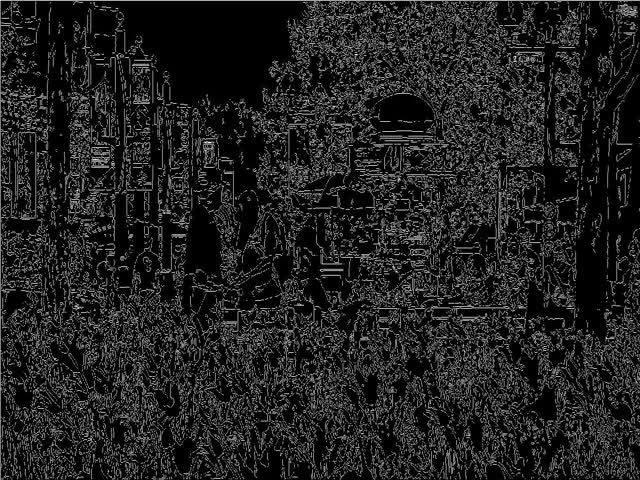
\includegraphics[ height=4cm, width=7cm]{spatialAC}}
\captionof{figure}{Przykład detekcji krawędzi obiektów w ramce, niezbędne do otrzymania informacji o aktywnosci przestrzennej \cite{agh_vqm}.}
\label{fig:xccs}
\end{center}


\item Letterbox i Pillarbox -- letterbox jest techniką pozwalającą na wyświetlanie obrazów o wyższym współczynniku proporcji na odbiornikach o mniejszym współczynniku. Polega ona na dołożeniu dwóch czarnych pasów na górze i dole ramki \cite{letterboxing}. Natomiast pillarbox używane jest przy wyświetlaniu obrazu o mniejszym współczynniku proporcji na ekranie o większym tymże współczynniku. Do obrazu dodawane są wtedy pasy po obu bokach ekranu. Skala przyjęta w pracy 0-1.
\begin{figure}[h]
\begin{subfigure}[b]{0.4\textwidth}
\centerline{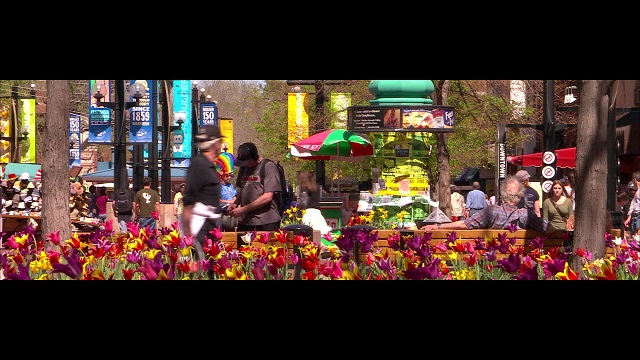
\includegraphics[ height=4cm, width=7cm]{letterboxingC}}
\caption{przykład wykorzystania techniki letterbox \cite{agh_vqm}.}
\label{fig:xccs}
\end{subfigure} 
\hfill
\begin{subfigure}[b]{0.4\textwidth}
\centerline{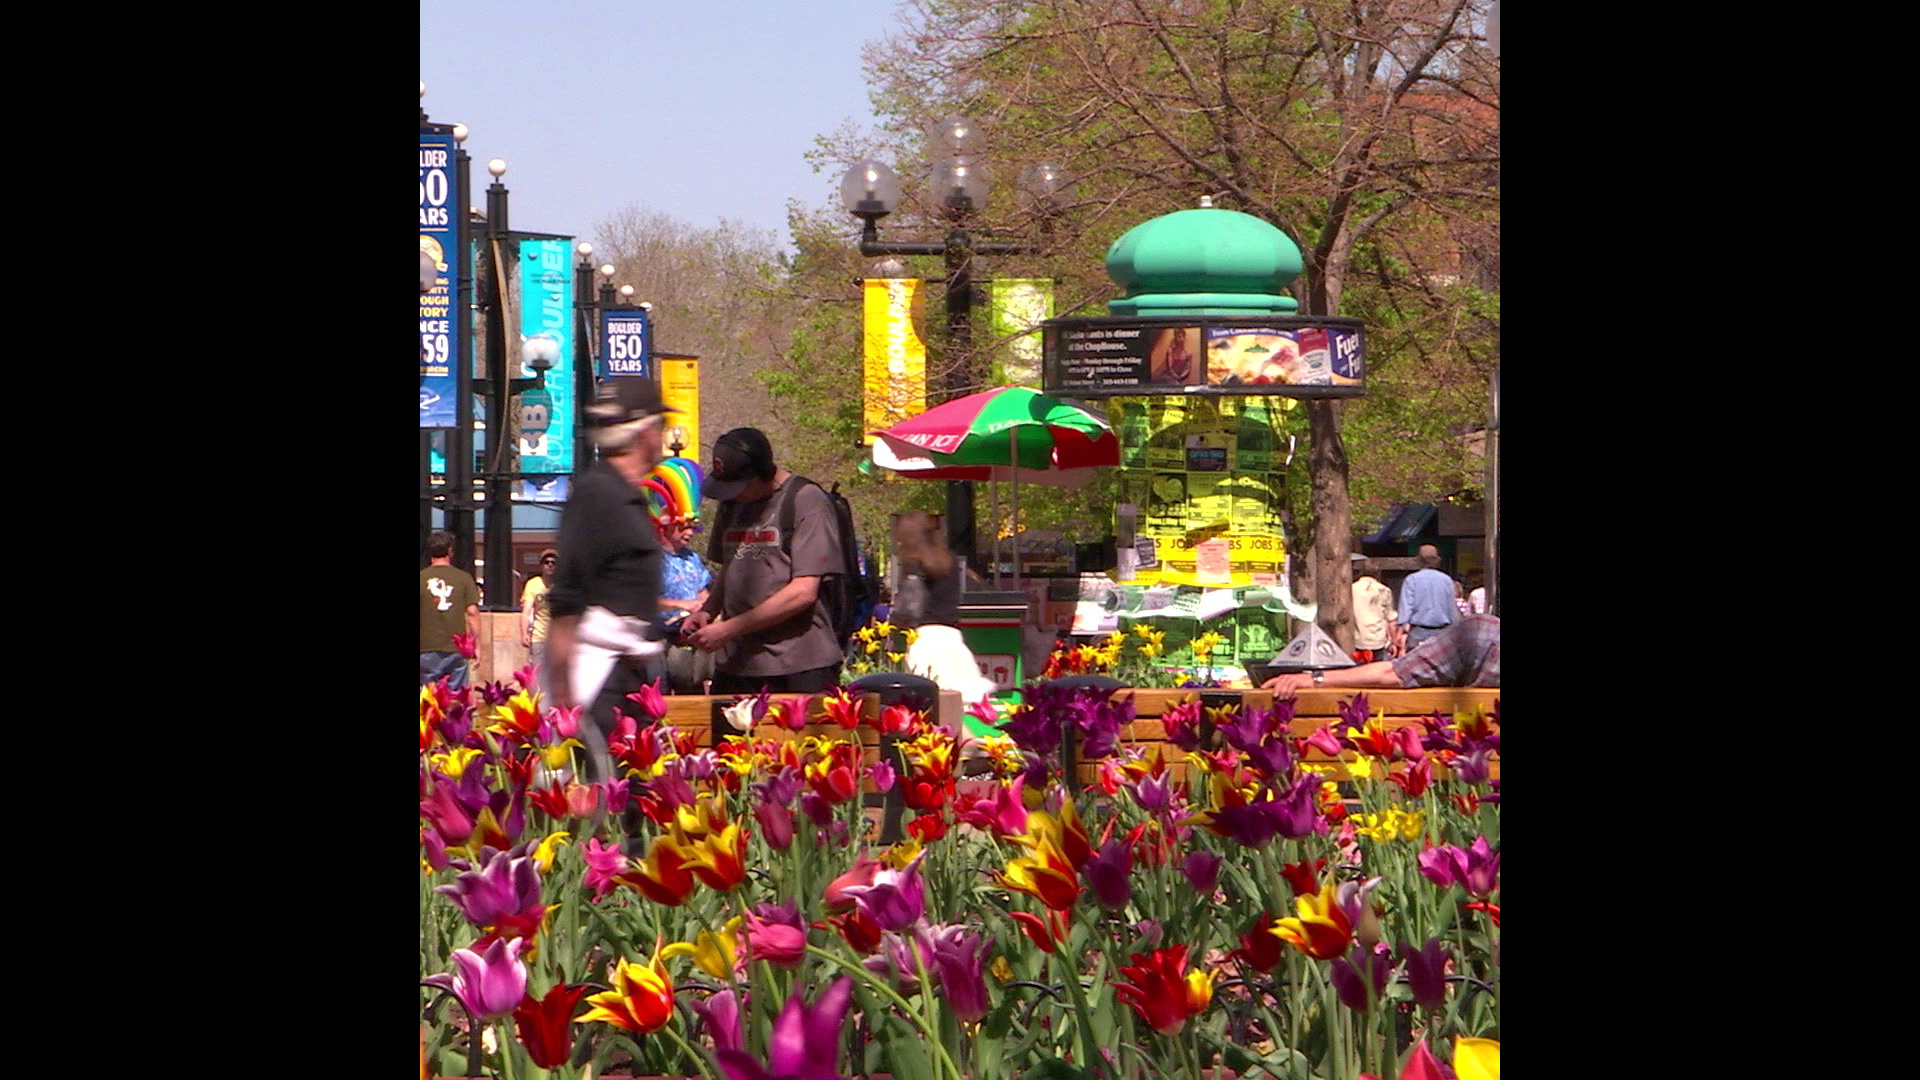
\includegraphics[ height=4cm, width=7cm]{pillarboxing}}
\caption{przykład wykorzystania techniki Pillarbox \cite{agh_vqm}.}
\label{fig:xccs}
\end{subfigure}
\end{figure}

\item Straty bloków ({\em ang. Blockloss}) -- wskaźnik informujący o ilości brakujących bloków (używanych podczas DCT/IDCT ), przykładowo zagubionych podczas transmisji skompresowanych danych. Skala przyjęta w pracy: 0-200. Im większa wartość tym większe zniekształcenie obrazu.


\begin{center}
\centerline{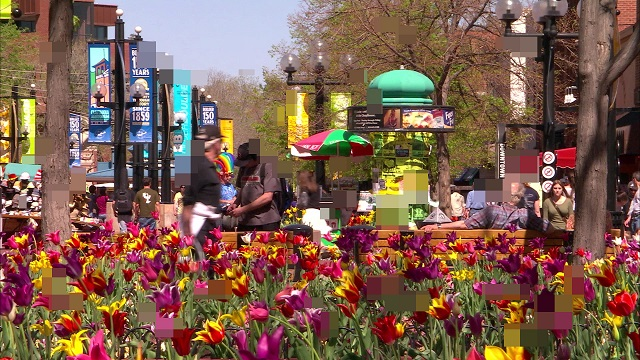
\includegraphics[ height=4cm, width=7cm]{block_lossC}}
\captionof{figure}{Przykład zniekształcenia obrazu spowodowany stratą bloków \cite{agh_vqm}.}
\label{fig:xccs}
\end{center}

\item Rozmycie ({\em ang. Blur}) -- Istnieje wiele rodzajów rozmycia, między innymi te niepożądane, występujące na przykład  po przeprowadzeniu kompresji z błędami, bądź przez poruszenie kamery podczas nagrywania. Gdy występuje ten efekt obiekty na obrazie tracą ostrość krawędzi \cite{blur}. Skala przyjęta w pracy: 0-70.
\begin{center}

\includegraphics[ height=4cm, width=7cm]{blur}
\captionof{figure}{Przykład zniekształcenia obrazu spowodowany rozmyciem \cite{agh_vqm}.}
\label{fig:xccs}
\end{center}

\item Aktywność czasowa ({\em ang. Temporal Activity}) -- opisuje intensywność ruchu obiektów w czasie. Często wymieniana razem ze wskaźnikiem aktywności przestrzennej. Skala przyjęta w pracy: 0-255.
\begin{center}
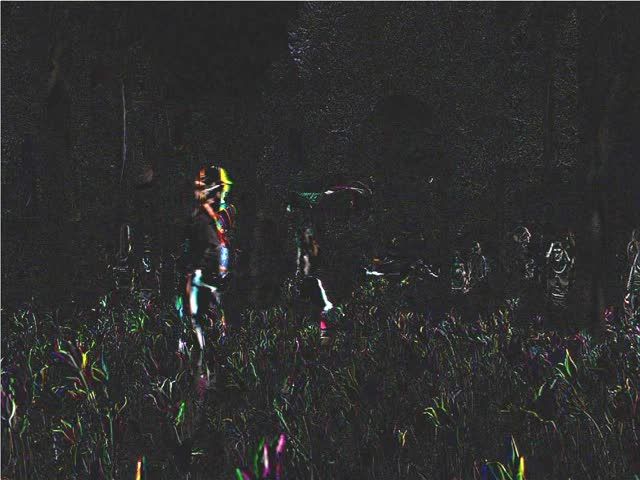
\includegraphics[ height=4cm, width=7cm]{temporalAC}
\captionof{figure}{opis}
\label{fig:xccs}
\end{center}

\item Wyciemnienia ({\em ang. Blackout}) -- opisuje zjawisko, kiedy obraz całkowicie zanika \cite{blackout}. Skala przyjęta w pracy : 0-1. \todo{sprzwdzic strony w i3e}
%\begin{center}
%
\includegraphics[ height=4cm, width=7cm]{blackout}
%\captionof{figure}{Wyciemniona ramka \cite{agh_vqm}.}
%\label{fig:xccs}
%\end{center}

\item Zamrożenie ({\em ang. Freezing}) -- Informuje o efekcie czasowego zatrzymania  obrazu,  które powoduje odczucie "przycięcia"  wideo \cite{freezing}. Transmitowana jest wtedy poprzednia poprawnie zdekodowana ramka. Skala przyjęta w pracy:0-1.

\item Ekspozycja ({\em ang. Exposure}) -- ten typ zakłóceń jest spowodowany niezbilansowaną jasnością ramek. Widz ma odczucie, że wideo jest zbyt ciemne lub zbyt jasne \cite{freezing}. Skala przyjęta w badaniach 0-255.
\begin{center}
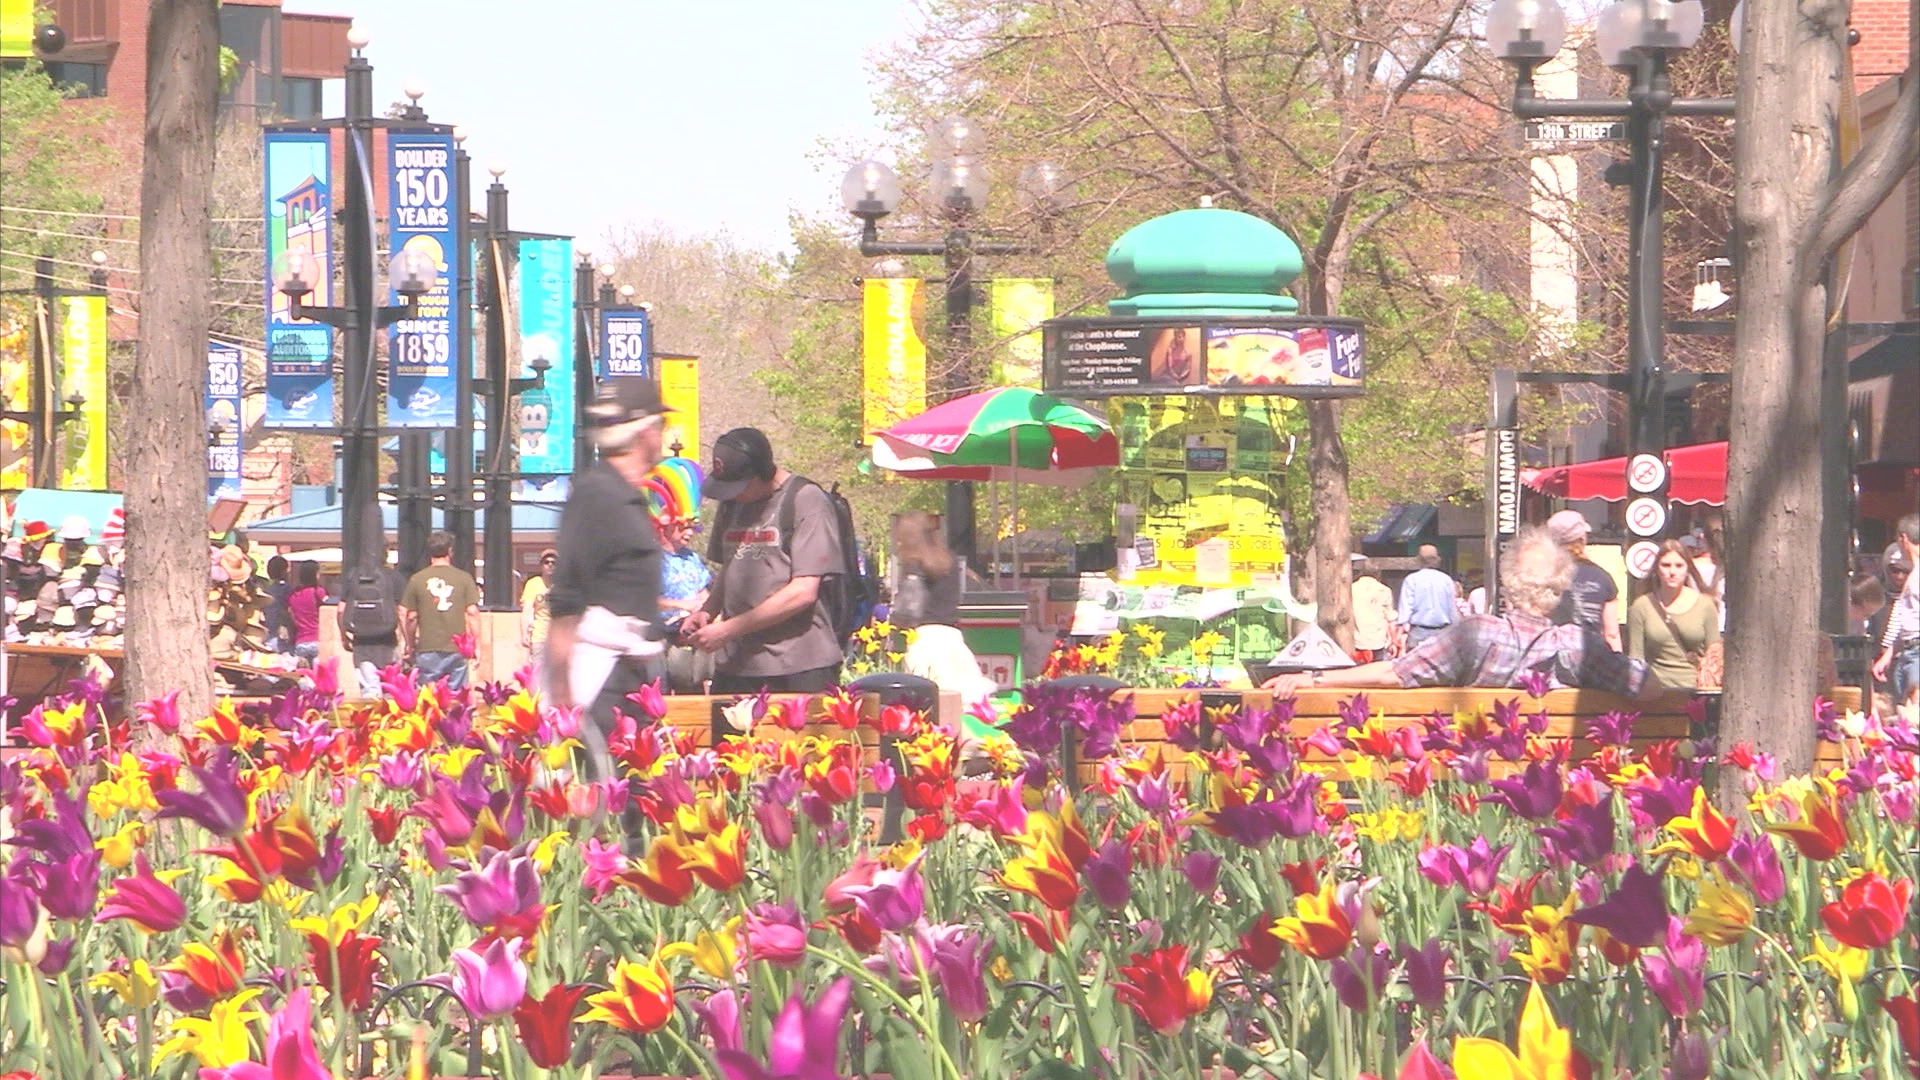
\includegraphics[ height=4cm, width=7cm]{exp}
\captionof{figure}{Przykład zniekształcenia obrazu spowodowany nieodpowiednią ekspozycją \cite{agh_vqm}.}
\label{fig:xccs}
\end{center}


\item Kontrast ({\em ang. Contrast}) -- Opisuje różnice pomiędzy jasnymi, a ciemnymi obszarami obrazu. Skala przyjęta w pracy: 0-120.
\begin{center}
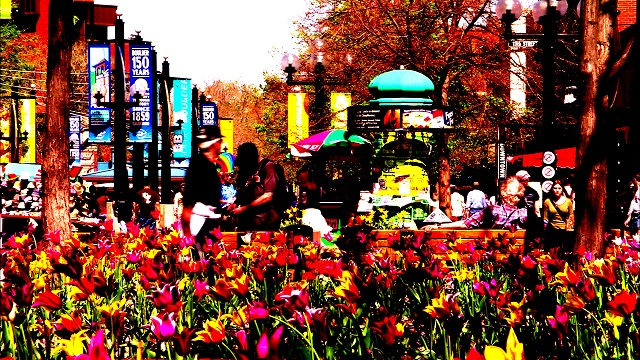
\includegraphics[ height=4cm, width=7cm]{contrastC}
\captionof{figure}{Przykład zniekształcenia obrazu spowodowany nieodpowiednim kontrastem \cite{agh_vqm}.}
\label{fig:xccs}
\end{center}
\item Jasność ({\em ang. Brightness}) -- jest powiązana z problemem ekspozycji. Jej zbyt duża wartość może skutkować odczuciem bladych kolorów w ramce. Skala przyjęta w pracy: 0-1.
\begin{center}
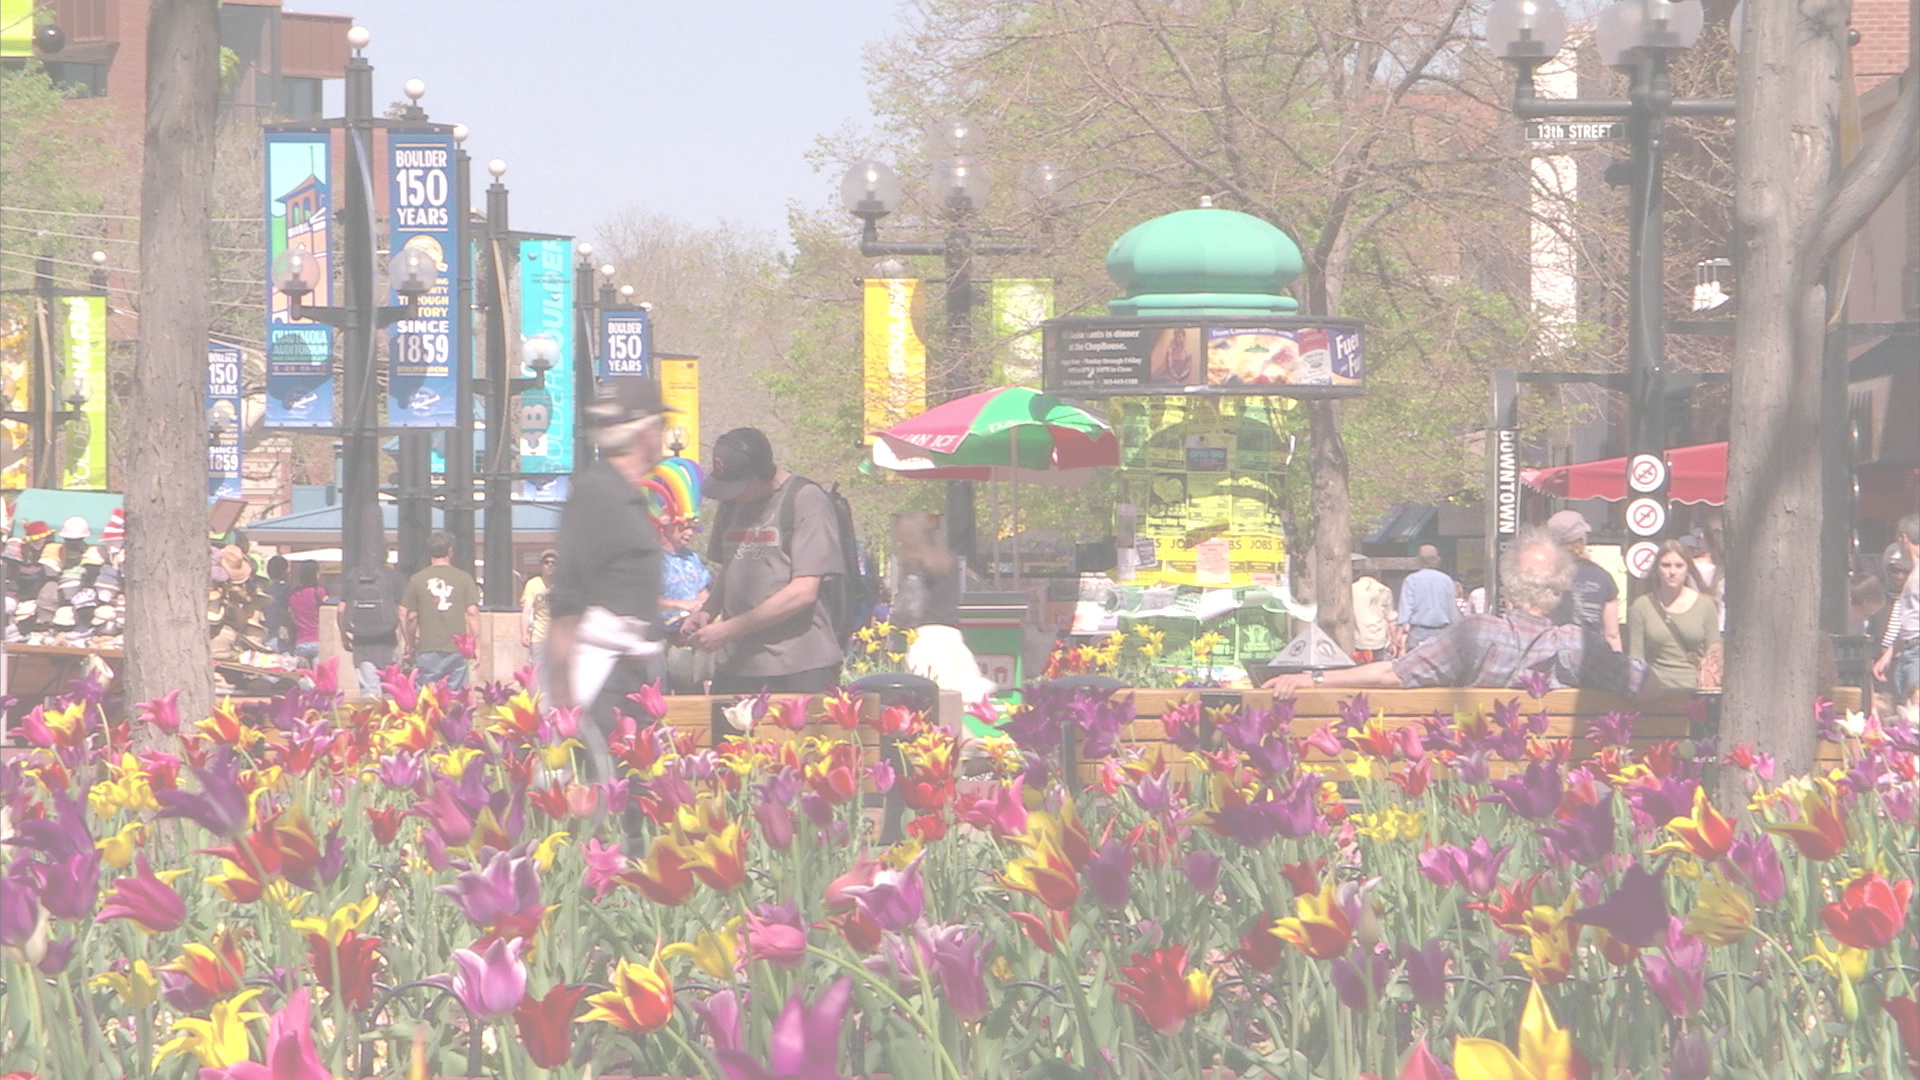
\includegraphics[height=4cm, width=7cm]{brightness}
\captionof{figure}{Przykład zniekształcenia obrazu spowodowany zbyt dużą jasnością \cite{agh_vqm}.}
\label{fig:xccs}
\end{center}

%\item interlace Skala przyjęta w pracy: 0-1.
%\begin{figure}[h]
%\centerline{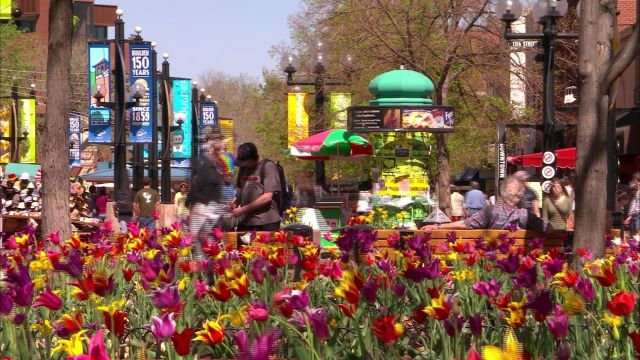
\includegraphics[ height=5cm, width=9cm]{interlace2C}}
%\caption{opis\cite{agh_vqm}}
%\label{fig:xccs}
%\end{figure}
\item Szum ({\em ang. noise}) -- jest to rodzaj zaburzenia obrazu spowodowany występowaniem niekontrolowanych wzorców dla intensywności wyświetlania pikseli \cite{freezing}. Skala przyjęta w pracy: 0-120.
\begin{center}
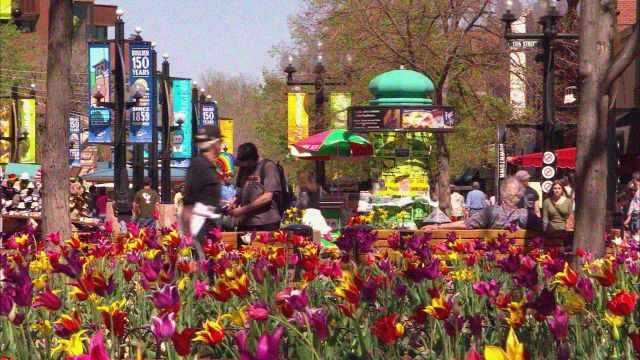
\includegraphics[ height=4cm, width=7cm]{noiseC}
\captionof{figure}{Przykład zniekształcenia obrazu spowodowany szumem \cite{agh_vqm}.}
\label{fig:xccs}
\end{center}

%\item Pocięcie ({\em ang. Slice}) -- objawia się efektem niepasujących do całości poziomych pasów. Związane jest to utratą pakietów danych podczas transmisji wideo. NIE DZIALA POPRAWNIE! 
%\begin{center}
%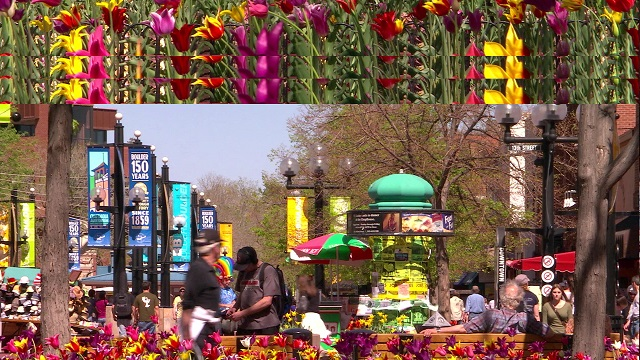
\includegraphics[ height=5cm, width=9cm]{slicingC}
%\captionof{figure}{A non-floating figure \emph{with} a caption!}
%\label{fig:xccs}
%\end{center}

\end{itemize}

Oprócz wyżej wymienionych wskaźników, w obecnym opracowaniu w pracy zostały również użyte dane o wideo, takie jak: 

\begin{itemize}[label=$\bullet$]
\item Rozdzielczość ({\em ang.  Resolution}) -- miara określająca rozmiar ramki. Jednostką są piksele. Podawana jest zazwyczaj w następujący sposób: szerokość x wysokość. Do badań zostały użyte wideo o rozdzielczościach: 3840x2160, 1920x1080, 704x576, 640x480, 352x288. 
\item Klatki na sekundę ({\em ang. fps, frames per second}) -- liczba ramek wyświetlonych w czasie sekundy. W telewizji stosowane jest 25 ramek na sekundę. Do badań użyto następujące częstotliwości: 60, 30, 25, 24 fps.
\item Próbkowanie chrominacji  ({\em ang.Chroma subsampling}) -- Jest to cecha  wideo wynikająca z sposobu kodowania  informacji w pikselu. \todo[inline]{To powinno być w opisie czym jest kompresja, jest to najczęściej pierwszy krok kompresji obrazu} Samo działanie ma na celu  ograniczenie zużycia zasobów.  W takim przypadku wykorzystuje się  niedoskonałość ludzkiego oka, które jest bardziej wrażliwe na jasność, niż na kolor. Jak wcześniej zostało wspominane piksel jest opisywany dwoma zmiennymi: luminacją i chrominacją. Piksel, w modelu kolorów YUV (innym modelem kolorów jest RGB),  jest  kodowany w następujący sposób: YCbCr, gdzie Y oznacza luminację, Cb intensywność koloru niebieskiego (chrominacja), a Cr intensywność koloru czerwonego (chrominacja). Chcąc zmniejszyć ilość danych, potrzebnych do zbudowania obrazu, ogranicza się informację dotyczące części odpowiedzialnej za kolor. Przykładowo 4:2:2 oznacza, że na daną czwórkę pikseli kolor będzie pod próbkowany na tylko co drugim z nich, a sąsiedzi przejmą od nich tą informację  \cite{chroma_sampling}. W danych zebranych do pracy użyto następujących wartości:.
\end{itemize}


\subsection{Metryki full-reference}

\begin{itemize}[label=$\bullet$]
\item PSNR ({\em ang. Peak Signal-to-Noise Ratio}) -- prosta do policzenia i również często stosowana z pomiędzy metryk typu FR. Przykładowa implementacja dla PSNR jest opisana wzorem  \ref{eqn:somelabel} (gdzie MSE jest błędem średnio kwadratowym dla ramki, $N$ ich liczbą, a $L$ maksymalną wartością sygnału). W pierwszej kolejności liczone jest zniekształcenie dla wszystkich ramek w stosunku do ich oryginału. Zazwyczaj do obliczań wykorzystuje się wyłącznie informację o luminacji piksela. Później następuje uśrednienie wyniku na wszystkie ramki\cite{fr_psnr}. 
\begin{equation}
\label{eqn:somelabel}
PSNR = \frac{1}{N} \cdot 10 \sum_{i=1}^{N}\log\frac{L}{MSE_i}
\end{equation}
Mimo zalet PSNR nie zawsze spełnia swoje zadanie. Ilustracja \ref{fig:psnr_pict} przedstawia w różny sposób zniekształcone obrazy. Każdy z nich otrzymał tą samą ocenę PSNR, a jednak ocena subiektywna wskazuje na różny poziom jakości.
\begin{center}
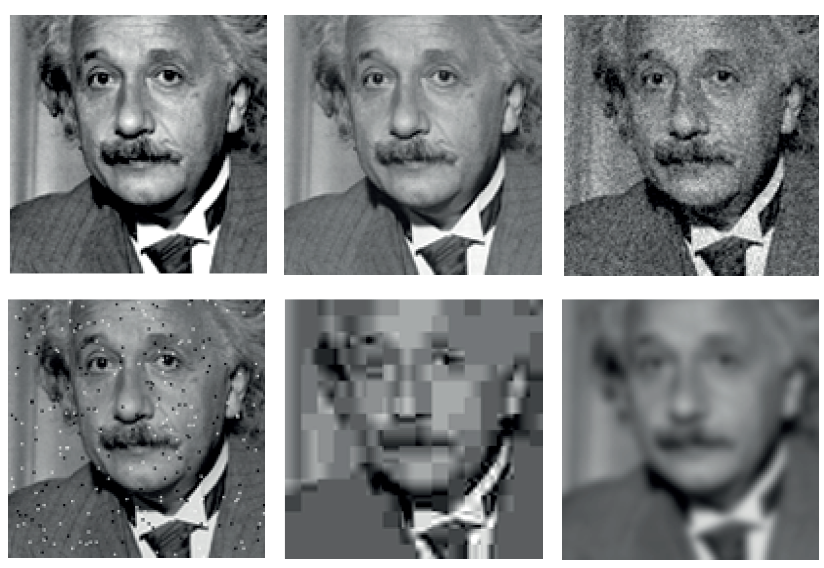
\includegraphics[ height=6cm, width=9cm]{psnr_pict}
\captionof{figure}{Wszystkie obrazy posiadają tą samą wartoć MSE \cite{psnr_qoe}.}
\label{fig:psnr_pict}
\label{fig:xccs}
\end{center}
% ms-ssim Multiscale_structural_similarity_for_image_quality_assessment
\item SSIM ({\em ang. Structural Similarity Index}) -- jest jedną z najczęściej stosowanych metryk oceny jakości wideo. Również, jak w poprzedniej metryce, zaletą jest prostota obliczeń. Uwzględnia w swojej funkcji \ref{eqn:ssim}: luminacje, kontrast i strukturę obu , gdzie S jest blokiem pikseli z ramki z oryginalnej sekwencji wideo, a S' jej zniekształconą wersją. $SSIM \in <0,1>$. 1 oznacza brak zniekształceń, a 0 idealne niedopasowanie \cite{ssim_1}\cite{ssim_2}.
\begin{equation}
\label{eqn:ssim}
SSIM = I(S, S')c(S, S')s(S,S')
\end{equation}
\item MS-SSIM ({\em ang. multi-scale SSIM}) -- jest modyfikacją poprzedniej metryki. Polega na próbkowaniu obrazu, w każdej skali, przed zastosowaniem SSIM'. Po przeprowadzeniu obliczeń, każda z skali jest łączona, z odpowiednimi wagami, w jedną całość. Zabieg ma na celu poprawę trafności oceny jakości \cite{ssim_2}. 
\item VMAF ({\em ang. Video Multimethod Assessment Fusion}) -- metryka rozwijana przez Netflix we współpracy z University of Southern California. Jej działanie opiera się na połączeniu wyników kilku metryk podstawowych. VMAF nadaje każdej z nich odpowiednie wagi, a dzieje się to dzięki zastosowaniu algorytmu uczenia maszynowego, w tym przypadku SVM regressor ({\em ang. Support Vector Machine regressor}). Takie rozwiązanie ma zapewnić wykorzystanie mocnych stron poszczególnych metryk z pominięciem ich słabości \cite{netflix}. 
\end{itemize}

\section{Algorytmy uczenia maszynowego }



%Obecne czasy charakteryzują się ogromną ilością danych. Coraz więcej dziedzin życia  które zewsząd otaczają człowieka i jego środowisko. \todo[inline]{To super dziwne zdanie, dane są jak powietrze?} W każdej sekundzie różnego rodzaju dane są zbierane, przesyłane, prezentowane i analizowane. Aby móc, w optymalny sposób, czerpać z nich zyski zostały opracowane pewne algorytmy, bazujące na statystyce. Algorytmy te potrafią zamodelować zadane zdarzenie i na jego podstawie dokonać predykcji . Mogą również w czasie rzeczywistym (czasem nawet korzystając ze swoich już dokonanych obliczeń), poprawiać i udoskonalać swoją strukturę zwiększając dokładność. Dziedzina nauki zajmująca się takimi algorytmami nazywana jest uczeniem maszynowym ({\em ang. Machine Learning}).\par \todo[inline]{To zupełnie nie tak. Pomieszanie systemów czasu rzeczywistego i ML i coś z danymi to straszne zagmatwanie i mijanie się z tym co jest istotne w pracy. W pracy chcemy powiedzieć, że 1. możliwości pozyskiwania i gromadzenia danych rosną, 2. narzędzia do ich przetwarzania są rozwijane bardzo intensywnie przez wiele różnych zespołów 3. ML pozwala tworzyć wiedzę w oparciu o dane (to istota ML!) 4. ML staje się coraz istotniejszym sposobem przetwarzania danych, gdzie wyciągamy wiedzę z danych bez naszego udziału}

 \todo[inline]{To zupełnie nie tak. Pomieszanie systemów czasu rzeczywistego i ML i coś z danymi to straszne zagmatwanie i mijanie się z tym co jest istotne w pracy. W pracy chcemy powiedzieć, że 1. możliwości pozyskiwania i gromadzenia danych rosną, 2. narzędzia do ich przetwarzania są rozwijane bardzo intensywnie przez wiele różnych zespołów 3. ML pozwala tworzyć wiedzę w oparciu o dane (to istota ML!) 4. ML staje się coraz istotniejszym sposobem przetwarzania danych, gdzie wyciągamy wiedzę z danych bez naszego udziału- DONE}

Obecne czasy charakteryzują się ogromną ilością danych. Jedną z nowszych koncepcji wprowadzanych w świat teleinformatyki, która się do tego przyczynia, jest Internet Rzeczy (\textit{ang. Internet of Things --  IoT}). Zakłada on, że urządzenia wyposażone w sensory komunikują się oraz wymieniają dane z innymi urządzeniami poprzez różnego rodzaju sieci. Co więcej styl życia obecnego społeczeństwa znacząco wpływa na  ciągłe powiększanie się istniejących baz danych i tworzenie nowych. Część codziennych czynności, jak na przykład przeglądanie  wiadomości czy w pewnym stopniu rozrywka, przeniosła się do sfery cyfrowej, dzięki technologiom i szerokiemu dostępowi do Internetu. Prowadzone są rejestry ruchu sieciowego i zachowań użytkowników. W ten sposób oraz dzięki wielu innym źródłom, różnego rodzaju dane są zbierane i gromadzone. Ten ciągle rosnący trend skłonił naukowców do badań na  mechanizmami pozwalającymi czerpać z nich zyski w bardziej optymalny sposób. Rozwiązaniem dla tych rozważań stały się algorytmy oparte na statystyce, które są w stanie zamodelować zadane zdarzenie i na jego podstawie dokonywać predykcji. Dziedzina nauki zajmująca się nimi nazywana jest uczeniem maszynowym ({\em ang. Machine Learning}). Mimo, że początki badań nad tymi algorytmami  przypadają na lata pięćdziesiąte ubiegłego wieku, to dopiero w najnowszych czasach zyskały one dużą popularność i zaczęły być stosowane przez komercyjne firmy. \par  


Jednym z zadań algorytmów uczenia maszynowego, jest odnalezienie jak najdokładniejszego przybliżenia funkcji: $f \colon X \to Y$. 
\todo[inline]{To eleiminuje algorytmy bez nauczyciela, reinforsment learning, oraz wiele algorytmów, gdzie Y nie jest tak jasno określone, jak tłumaczenie. W pracy trzeba być precyzyjnym i opisać dokładnie o co chodzi.- done?}
 Jest to funkcja opisująca zależności pomiędzy danymi wejściowymi $X$, a danymi wyjściowymi $Y$ \cite{ml_supervised}. Ten przypadek będzie również rozważany w obecnej pracy. Do oceny poprawności tak przygotowanych modeli korzysta się między innymi z współczynnika determinacji R-kwadrat ($R^2$) pokazuje on jak bardzo udało się zbliżyć do tej funkcji. Definiowany jest on wzorem \ref{eqn:r2}. 
\begin{equation}
\label{eqn:r2}
R^2=1- \frac{ \sum_{i=1}^{n}(y_i-y'_i)^2}{\sum_{i=1}^{n}(y_i-\bar{y}_i)^2 }
\end{equation}
Gdzie, $y_i$ oznacza rzeczywistą wartość szukanej przez model zmiennej, $y'_i$ predykcję modelu, $\bar{y_i}$ średnią wartość dla wszystkich $y_i$. Przykładowo 1 oznacza idealne dopasowanie modelu, 0 oznacza, że model jest tak samo dokładny jak wartość średnia.\par
Dalsze  podrozdziały będą również zawierać krótki opis algorytmów użytych do badań w niniejszej pracy.

\subsection{Ucznie nadzorowane i nienadzorowane}
Wyróżniane są dwa typy algorytmów uczenia maszynowego: nadzorowane ({\em ang. supervised learning}) i nienadzorowane ({\em ang. unsupervised learning}). Różnica występuje podczas procesu tworzenia modelu -- trenowania. W pierwszej grupie, w celu poprawnego zbudowania modelu, wymagane jest, aby dane treningowe składały się z par: dane wejściowe i odpowiadające im  dane wyjściowe (nazywane nauczycielem). Druga grupa nie wykorzystuje danych wyjściowych podczas trenowania. W badaniach zostały użyte algorytmy z uczeniem nadzorowanym. Kolejne rozdziały będą odnosić się do tej właśnie grupy. \par 

\subsection{Problem klasyfikacji i regresji}
W ramach algorytmów uczenia maszynowego z uczeniem nadzorowanym wyróżnia się dwa typy rozważanych  problemów: regresji i klasyfikacji (\textit{ang. classification and regression task}). Dla tych pierwszych model ma za zadanie mapować dane wejściowe na skończony zbiór danych wyjściowych. Przykładem wykorzystania klasyfikacji binarnej jest rozpoznawanie spamu w poczcie elektronicznej. Algorytmy dla problemu regresji dokonują estymaty funkcji opisującej zależności danych wejściowych i ciągłego zbioru danych wyjściowych. Przykładem może być predykcja temperatury \cite{rf2}.
W niniejszej  pracy rozpatrywany  jest problem regresji. \par



%(?czy wpisywac cos o metodzie uczenia zaimplementowanej w skLearn, czyli :Ordinary Least Squares ?)
\subsection{Regresja Liniowa}
W Regresji Liniowej w jej podstawowej postaci zmienna niezależna $x_i$ ({\em ang. independent variable}) opisuje zmienną zależną $y_i$ ({\em ang. dependent variable}) zgodnie z następującym wzorem $y_i = \beta_0 + \beta_1 x_i + \epsilon$. Gdzie $\beta_0$ i $\beta_1$ są współczynnikami określającym relację danych, czyli zmiennych $x$ i $y$. Do badań w pracy zostało wykorzystane pewne rozszerzenie klasycznej regresji liniowej -- wielokrotna regresja liniowa ({\em ang. Multiple Linear Regression}), gdzie $y_i$ jest opisany następującą zależnością \ref{eqn:regresja}. Oznaczenia poszczególnych elementów tego równania są analogiczne do podstawowej wersji regresji. Trenowanie takiego modelu polega na szukaniu współczynników $\beta$ \cite{mlr} .\par

\begin{equation}
\label{eqn:regresja}
y_i = \beta_0 + \beta_1 x_{1i} + \beta_2 x_{2i} + ... + \beta_p x+x_{pi} + \epsilon
\end{equation}

Regresja liniowa jest jednym z prostszych algorytmów. Jej cechą jest przejrzystość w interpretacji  dzięki możliwości obserwacji współczynników $\beta$. Regresja liniowa jest w stanie odnajdować zależności liniowe, natomiast dla zależności nieliniowych może dawać fałszywe wyniki.

\subsection{SVM}
{\em Software Vector Machine} (SVM) -- algorytm używany jako klasyfikator, który dokonuje podziału danych dzięki wcześniej wyznaczonej hiperpłaszczyźnie ({\em ang. hyperplane}). Upraszczając dla przestrzeni dwuwymiarowej, w celu zdefiniowania optymalnej hiperpłaszczyzny należy wyznaczyć maksymalną szerokość marginesów ({\em ang. margin} ) $\omega$, taką aby dane z różnych klas były od siebie oddzielone oraz, aby pojedyncze dane z różnych klas, znajdujące się najbliżej siebie, leżały na granicy marginesów (jak na rysunku \ref{fig:svm} ).  Takie dane definiowane są jako {\em ang. Support vectors}. Wielu przypadkach, aby podział danych był możliwy, używa się  jednej z funkcji kernela, przenoszącej problem do przestrzeni złożonej z większej liczby wymiarów. Rysunek \ref{fig:svm} przedstawia przykładową hiperpłaszczyznę.\par

%NOWY OBRAZEK https://en.proft.me/2014/04/22/how-simulate-support-vector-machine-svm-r/
\begin{center}
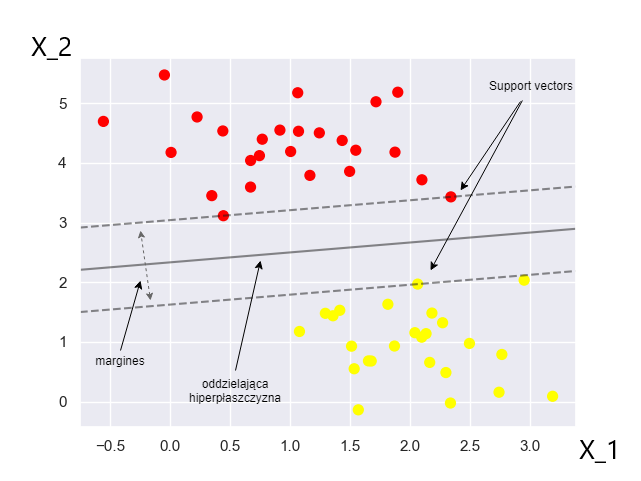
\includegraphics[ height=10cm, width=13cm]{svm_2}
\captionof{figure}{Hiperpłaszczyzna rozdzielająca dane, o dwóch właściwościach $x_1$ i $x_2$, na dwie klasy: czerwoną i żółtą}
\label{fig:svm}
\label{fig:xccs}
\end{center}

W niniejszej pracy zostało użyte pewne rozwinięcie SVM, dla problemów dotyczących regresji, czyli SVR ({\em ang. Support Vector Regression}). W takim rozwiązaniu hiperpłaszczyznę wyznacza się tak, aby jak najwięcej danych treningowych znalazło się w wybranej odległości $\epsilon$ od niej, w celu dopasowania funkcji $f \colon X \to Y$ \cite{svr}. Zaletą SVM i SVR jest to, że są w stanie odnajdywać zależności nieliniowe, jednak by tego dokonać należy wybrać odpowiednią funkcję kernala, co często nie jest trywialne.

%SVR -> https://link.springer.com/chapter/10.1007/978-1-4302-5990-9_4
\subsection{Las Losowy}
Las Losowy (\emph{ang. Random Forest -- RF}) działa w oparciu o "głosowanie"' wielu pojedynczy drzew. Każde z drzew powstaje dzięki implementacji algorytmu CART ({\em ang. Classification and Regression Trees}). W tym przypadku dla problemów regresji. Drzewa składają się z węzła głównego ({\em ang. Root Node}), liści ({\em ang. Leaves}), węzłów decyzyjnych ({\em ang. Decision Nodes}). Trenowanie drzewa bazuje na minimalizacji funkcji $S$ wyrażającej się wzorem \ref{eqn:rf}, gdzie $m_c=\frac{1}{n}\sum_{i \in c}y_i'$ i jest predykcja z danego liścia \cite{rf}. Rysunek \ref{fig:r_tree} wizualizuje dopasowanie funkcji przy użyciu algorytmu  drzewa regresyjnego.\par
\begin{equation}
\label{eqn:rf}
S=\frac{1}{n}\sum_{c \in leaves(T)}\sum_{i \in c}(y_i - m_c)^2
\end{equation}

W RF każde z drzew budowane jest w oparciu o inny podzestaw danych treningowych, co w swoim zamyśle ma na celu podwyższenie dokładności modelu oraz zmniejszenie zagrożenia nadmiernego dopasowania ({\em ang. overfitting}) \cite{rf2}. Istotną kwestią jest dobór optymalnych parametrów dla modelu, takich jak liczba drzew oraz ich głębokość. 
\begin{center}
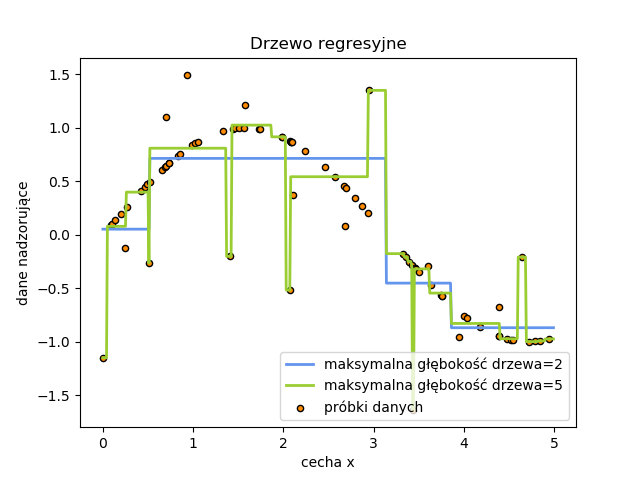
\includegraphics[ height=6cm, width=9cm]{r_tree}
\captionof{figure}{Wizualizacja dopasowania modelu z użyciem algorytmu drzewa regresyjnego.}
\label{fig:r_tree}
\label{fig:xccs}
\end{center}

\subsection{Sieci Neuronowe}
Struktura Sieci Neuronowych ({\em ang. Neural Networks}) jest inspirowana budową mózgu. Jej podstawowym elementem są neurony, które formują warstwy, te z kolei dzielą się na warstwę wejściową, warstwę wyjściową i warstwy ukryte. Rysunek \ref{fig:nn} przedstawia schemat przykładowej sieci neuronowej jednokierunkowej (\textit{ang. feedforward}). Ten typ został również wybrany do eksploracji danych w obecnym opracowaniu. 

Każdy pojedynczy neuron działa jak funkcja $ \sigma :\mathbb{R} \to \mathbb{R}$, nazywana jest ona  funkcją aktywacji. Przykłady tak stosowanych funkcji to funkcja: sigmoidalna, progowa czy ReLU. Tak zamodelowane neurony jako dane wejściowe otrzymują dane wyjściowe, z odpowiednią wagą, z poprzednich neuronów. Neurony z warstwy wejściowej otrzymują przygotowane dane treningowe \cite{rf2}. Proces uczenia, który ustawia wagi, a tym samym mówi jak powinny wyglądać połączenia pomiędzy neuronami w różnych warstwach, nosi nazwę {\em Back Propagation} \cite{bp}.\par


\begin{center}
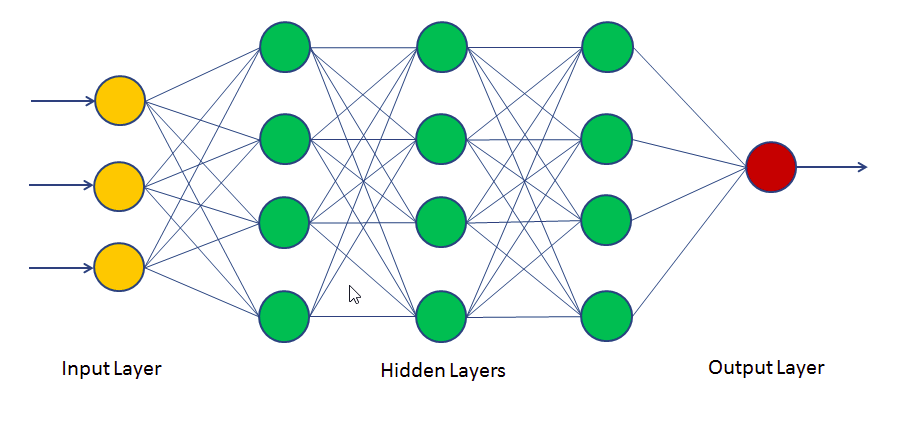
\includegraphics[ height=6cm, width=12cm]{nn}
\captionof{figure}{Przykładowy schemat budowy sieci neuronowej. Żółte koła symbolizują neurony z warstwy wejciowej, niebieskie i zielone neurony z warstw ukrytych, a czerwony neuron z warstwy wyjściowej \cite{nnpicture}. }
\label{fig:nn}
\label{fig:xccs}
\end{center}

Jedną z największych zalet sieci neuronowych jest to, że w porównaniu z innymi algorytmami uczenia maszynowego, w lepszym stopniu wykorzystują duże ilości danych wejściowych \cite{nndata}. Zależność ta została zobrazowana na wykresie \ref{fig:nn_data}. Co więcej algorytm ten dobrze radzi sobie z zależnościami nieliniowymi. Minusem natomiast jest utrudniona możliwość obserwacji jak algorytm doszedł do danego wyniku. Działa on jak pewnego rodzaju czarna skrzynka. Możliwa jest  sytuacja, kiedy predykcja modelu w żadnym stopniu nie wskazuje na rzeczywisty wynik. W takim przypadku bardzo trudny jest proces śledzenia kolejnych kroków jakie zostały wykonane po drodze i zrozumienia co jest jego przyczyną błędnej oceny. 
%00097934
%haykin.neural-networks.3ed.2009
%https://www.researchgate.net/publication/324728060_Lung_Cancer_Detection_using_Deep_Learning#pf18



\begin{center}
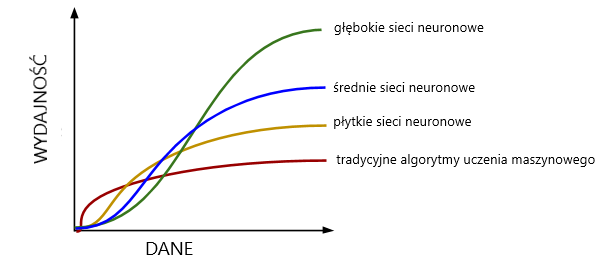
\includegraphics[ height=6cm, width=14cm]{nn_data_2}
\captionof{figure}{Wydajnosć sieci neuronowych w porównaniu do tradycyjnych algorytmów uczenia maszynowego \cite{nn_wykres}.}
\label{fig:nn_data}
\label{fig:xccs}
\end{center}







